\chapter{Introduction}
\section{Motivation}
A non-negligible amount of the total electricity consumed is due to residential and commercial illumination.
According to the U.S. Energy Information Administrator (EIA) about $7\%$ of the total electricity consumed in the U.S. in 2017 was for lighting \cite{}. These figures are impressive if one considers that the global electricity consumption was more than $20,000$ TWh in 2016 \cite{}. 

The energy consumed by an illumination device is clearly related to the efficiency of the device itself. 
In particular, part of the energy consumption constists of excessive, misdirected and inefficent use of light, which could be used in a smarter way. A tangible aspect of such lack of efficiency is light pollution, a persistent and increasing problem in most cities. Light pollution is wasted energy and can have adverse impacts on everything from humans’ sleep patterns to bird and fish migration to plants’ growth periods \cite{}. Figures \ref{fig:light_pollution} and \ref{fig:light_pollution2} show the light pollution of the Gulf of Naples.
\begin{figure}[t]
\centering
  \begin{minipage}[]{0.49\textwidth}
    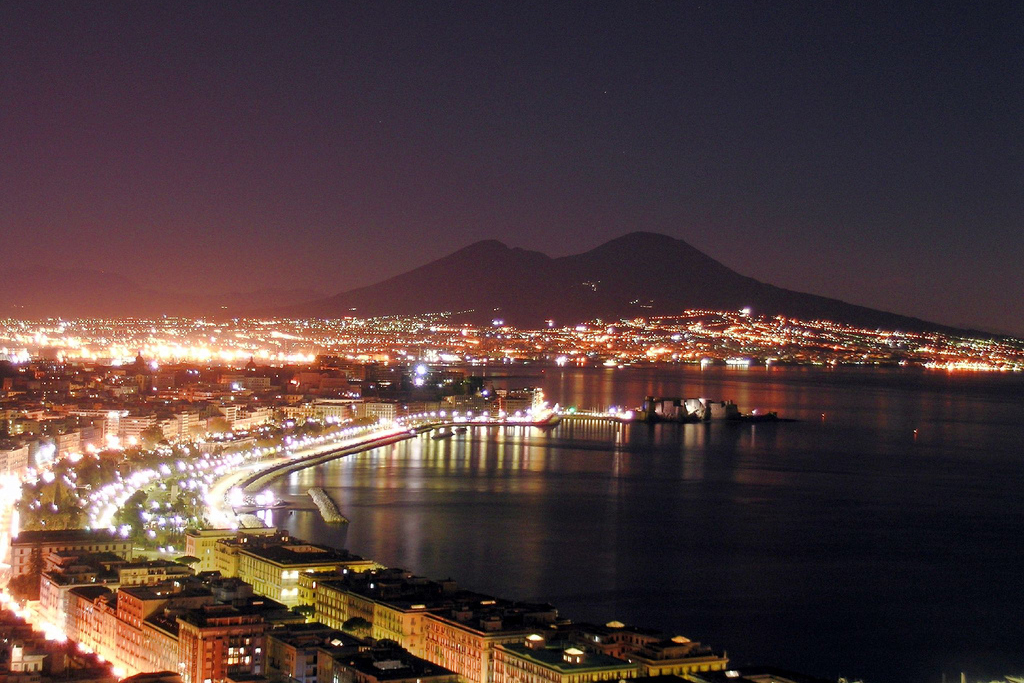
\includegraphics[width  = \textwidth]{gulf_naples}
    \caption{\textbf{Gulf of Naples at night \cite{}}}
    \label{fig:light_pollution}
\end{minipage}
\hfill
 \begin{minipage}[]{ 0.49\textwidth}
    \includegraphics[width  =\textwidth]{naples}
    \caption{\textbf{Satellite view of Naples \cite{}.}}
    \label{fig:light_pollution2}
\end{minipage}
  \end{figure}

Using efficient light sources could help to mitigate both the amount of energy consumption and light pollution.
Because of this, many optical industries are interested in fabricating efficient light sources.
Currently, light emitting
diodes (LEDs) are replacing traditional sources \cite{koshel2012illumination}. 
This is mainly due to their high energy efficacy and very long lifetime, \cite{taguchi2008present, haitz2011solid}. 
% Efficienza LED allungo il brodo
LED systems consist of several components. 
Electronic devices convert the AC mains voltage into a voltage suitable for the LED source.
An optical system is required, it is formed by optical components such as lenses and reflectors \cite{moreno2008modeling}. Light emitted from the LED propagates within the system which reshapes light according to physical laws (e.g. reflection, refraction and scattering phenomena). LED systems are increasingly used in many application such as street lights, automotive lighting and home illumination. 
However, the efficiency of the source does not reflect how much light is transferred from the source to the target, and for each application a certain target distribution is desired. For example, street lights should provide a uniform illumination of the streets; car headlights should be built such that they have a powerful and uniform light while avoiding uncomfortable glare for the oncoming traffic. The material and the shape of the optical systems are very important for the efficiency of the entire lighting system. Thus, our aim is to design an optical systems which directs light only where illumination is desired, avoiding to spread light everywhere.

Illumination optics is the branch of optics that deals with the design of optical systems. It concerns the transfer of light from the source to the target. The goal in illumination optics is to obtain the desired light distribution at the receiver after its propagation through the optical system. Depending on the intensity distribution required, an optical engineer can determine what type of optic is needed. To this purpose, it is important to understand how light propagates through a given optical system.

Light can be seen as the electromagnetic radiation perceived by the human eye \cite{schreuder2008outdoor}. Therefore, it propagates as an electromagnetic wave and, as such, it has a certain wavelength. Visible light has wavelength in the range between $400$ and $700$ nm. When light wavelength is incredibly small compared to the dimensions of the optics to which it interacts, it is reasonable to consider the limit of infinitely short wavelengths. The field of optics that discard the microscopic wave behavior of light is called \textit{geometric optics}. In the geometric optics approximation, light is described by rays that propagate perpendicular to the wavefront transporting electromagnetic energy. Since the dimensions of the optical components used for illumination systems are rather big compared to the wavelength of visible light, illumination optics is usually described in terms of geometrical optics. 

To compute the photometric variables at the target of the
optical system, the ray tracing procedure is widely used in the field of geometric optics \cite{glassner1989introduction}.
Ray tracing is a forward method which provides the light target distribution given a light source and an optical system \cite{Gross2005Handbook}. Every ray is considered to be a straight line when propagates in free space. Once it hits an optical surface its direction changes according to reflection and refraction law. Ray tracing computes the intersection points of every ray emitted from the source with \textit{all} the optical surfaces that it encounters. Next, it calculates the surfaces located at the closest distance from the point on which the ray was emitted. The new ray direction at the intersection point ray is computed. The procedure continues until the ray reach the target and it is repeated for all the rays traced.
There are many ways to implement the ray tracing process.

Monte Carlo (MC) ray tracing is often used in nonimaging
optics. This method is based on a probabilistic interpretation
of the rays distribution at the source of the optical
system \cite{liu2010precise,Ting:1}: many rays are traced randomly from the source,
and their distribution at the target is estimated to compute the
photometric variables of the output light. For example, the output intensity distribution is provided dividing the target into equal cells and counting on average the number of rays that arrive at each part of the target. Although the MC
procedure constitutes a robust method, it remains a slow and
numerically costly procedure, as it converges proportionally
to the reciprocal value of the square root of the number of rays
traced. Therefore, to obtain a good accuracy of the intensity distribution at the target million of rays need to be traced.

To speed up MC ray tracing, deterministic Quasi-Monte Carlo (QMC) ray tracing was introduced. The difference between MC and QMC is that in the latter the coordinates of the rays traced are distributed according to a \textit{low-discrepancy sequences}. Intuitively the discrepancy indicates how much the rays distribution differs from a uniform distribution.  Hence, low discrepancy sequences are close to uniformly distributed sequences \cite{levy2002introduction}.
In some cases QMC ray tracing is an improvement of MC ray tracing \cite{ohbuchi1996quasi, caflisch1998monte}. However, it is not possible to predict the convergence of QMC ray tracing as the error is always bounded by a term proportional to the discrepancy of the initial sample of rays. It has been proven that in some cases the performances of the two method are comparable \cite{tuffin2004randomization}.

The purpose of this thesis is to provide tools to improve illumination optics design by using faster and more accurate methods than the current state-of-the-art ray tracing methods.
To do so, we analyze optical systems using the \textit{phase space} concept \cite{torre2005linear}.
The phase space (PS) of an optical surface is described by the position and direction coordinates of all the rays that hit the surface \cite{testorf2009phase}. We restrict ourselves to the two-dimensional case which is particularly relevant as it constitutes a good test case to
demonstrate the performance of the new ray tracing method. For any rotational symmetric
system the 2D case is very useful to study. Optical designers often start working in two dimensions where only the
meridional plane is taken into account. In two dimensions we refer to \textit{optical lines} instead of optical surfaces. The PS of a two-dimensional system is a two-dimensional space described by all the possible ray positions and directions. 

Optical phenomena can be analyzed by using the PS and the photometric variables can be defined in PS \cite{rausch2014illumination}.  
%For example, the \'{e}tendue can be seen as the area covered by the rays in phase space which can be calculated either using numerical integration or, for very simple systems, even analytically. The luminance is the power distribution in phase space. For systems formed by a Lambertian source the output luminance is a positive constant when different from zero. The intensity is given by an integration of the luminance over all the possible positions in phase space. Assuming a Lambertian source, the intensity along every direction is simply the support of the luminance given by the sum of the distances between the rays located on the boundaries of the regions with positive luminance. 
Currently, some material based on phase space optics has been published, showing that light propagation can be investigated using the phase space concept \cite{rausch2012phase,rausch2014phase, herkommer2012phase}. Also, phase space optics might constitute an alternative approach for describing aberration phenomena \cite{herkommer2013phase, babington2017freeform, wolf1993relativistic}. In this thesis we introduce new methods based on PS providing a new way to calculate the light distribution at the target of optical systems. The PS methods significantly improve the performance of existing procedures used to this purpose in illumination optics, i.e., MC and QMC ray tracing. 
Next, the methods and results are briefly discussed. 
\section{Phase space methods and results}
The new methods presented in this thesis are based on PS rays tracing. The PS of a line is a $2$D space described by one position and one direction coordinate of the ray. 
The position coordinate is given by one of the two coordinates of the intersection point between the rays and the optical line, the direction coordinate is the sine of the angle that the ray forms with the normal of the line encountered measured counterclockwise multiplied by the index of refraction of the material in which the line is located \cite{wolf2004geometric}. In Figure \ref{fig:TIR_intro} we show a ray that follows a certain path when propagating inside an optical system. This ray corresponds to a unique point in PS. In Figure \ref{fig:PS_intro} we represent the ray traced at the target PS of the system.
\begin{figure}[t]
  \begin{minipage}[t]{0.49\textwidth}
\centering
    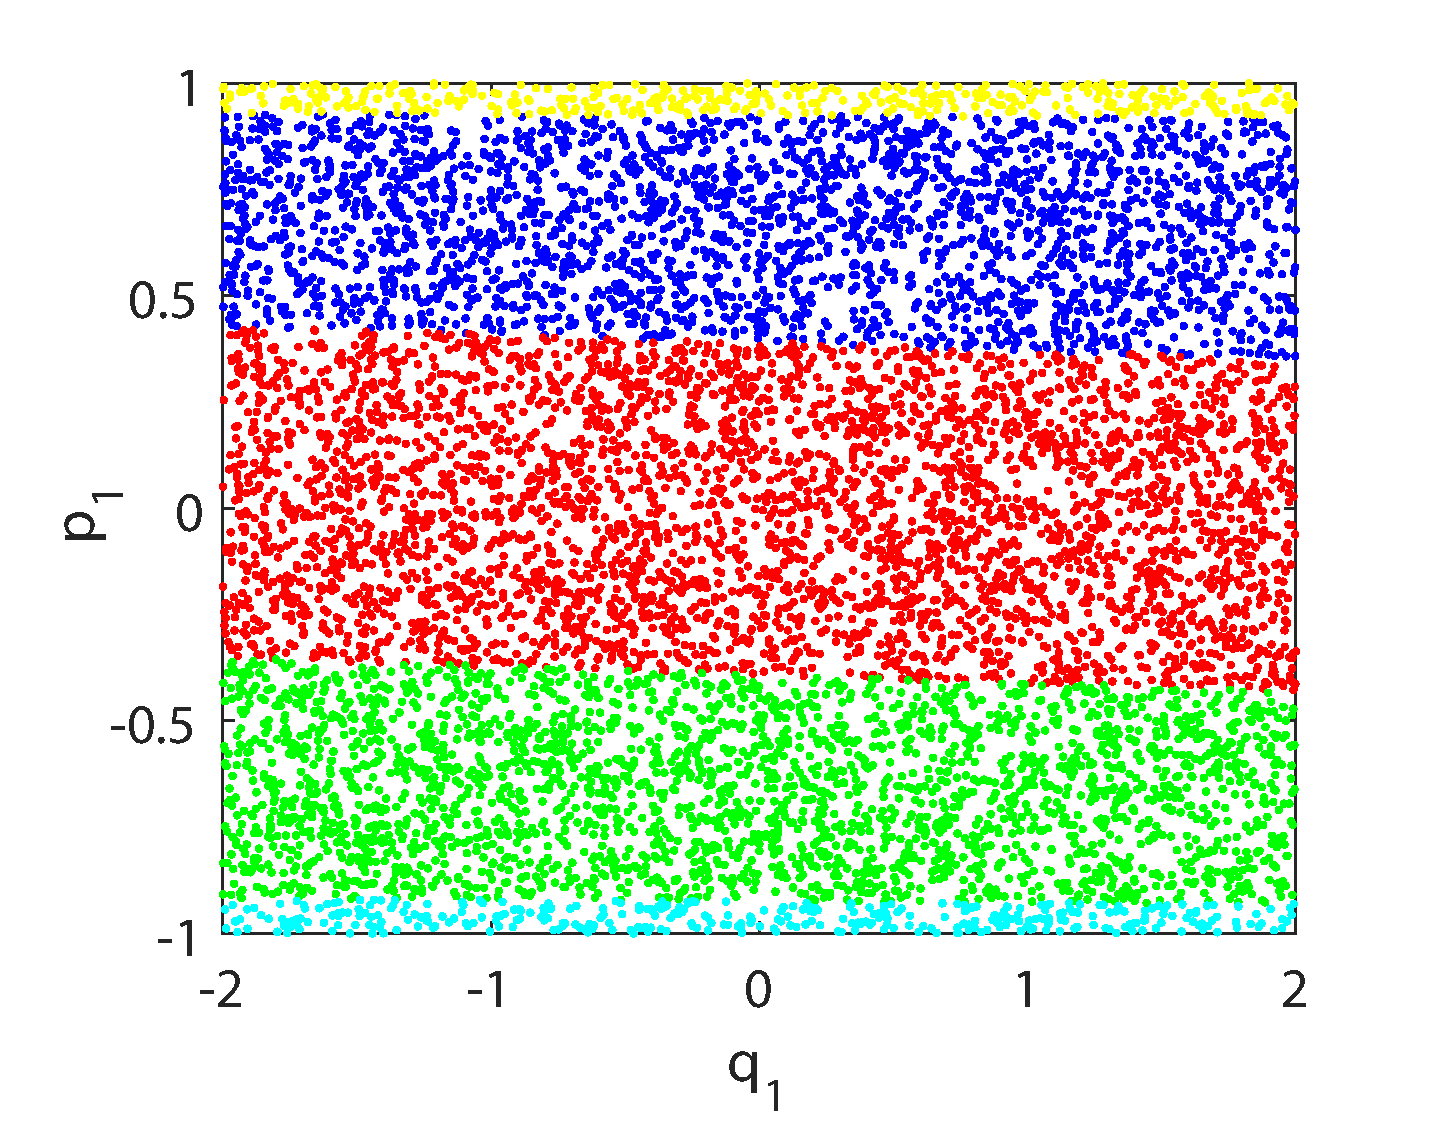
\includegraphics[width  = \textwidth]{source_PS_cup.pdf}
    \caption{\textbf{A ray propagating inside an optical system.}}
    \label{fig:TIR_intro}
  \end{minipage}
\hfill
  \begin{minipage}[t]{0.49\textwidth}
\centering
    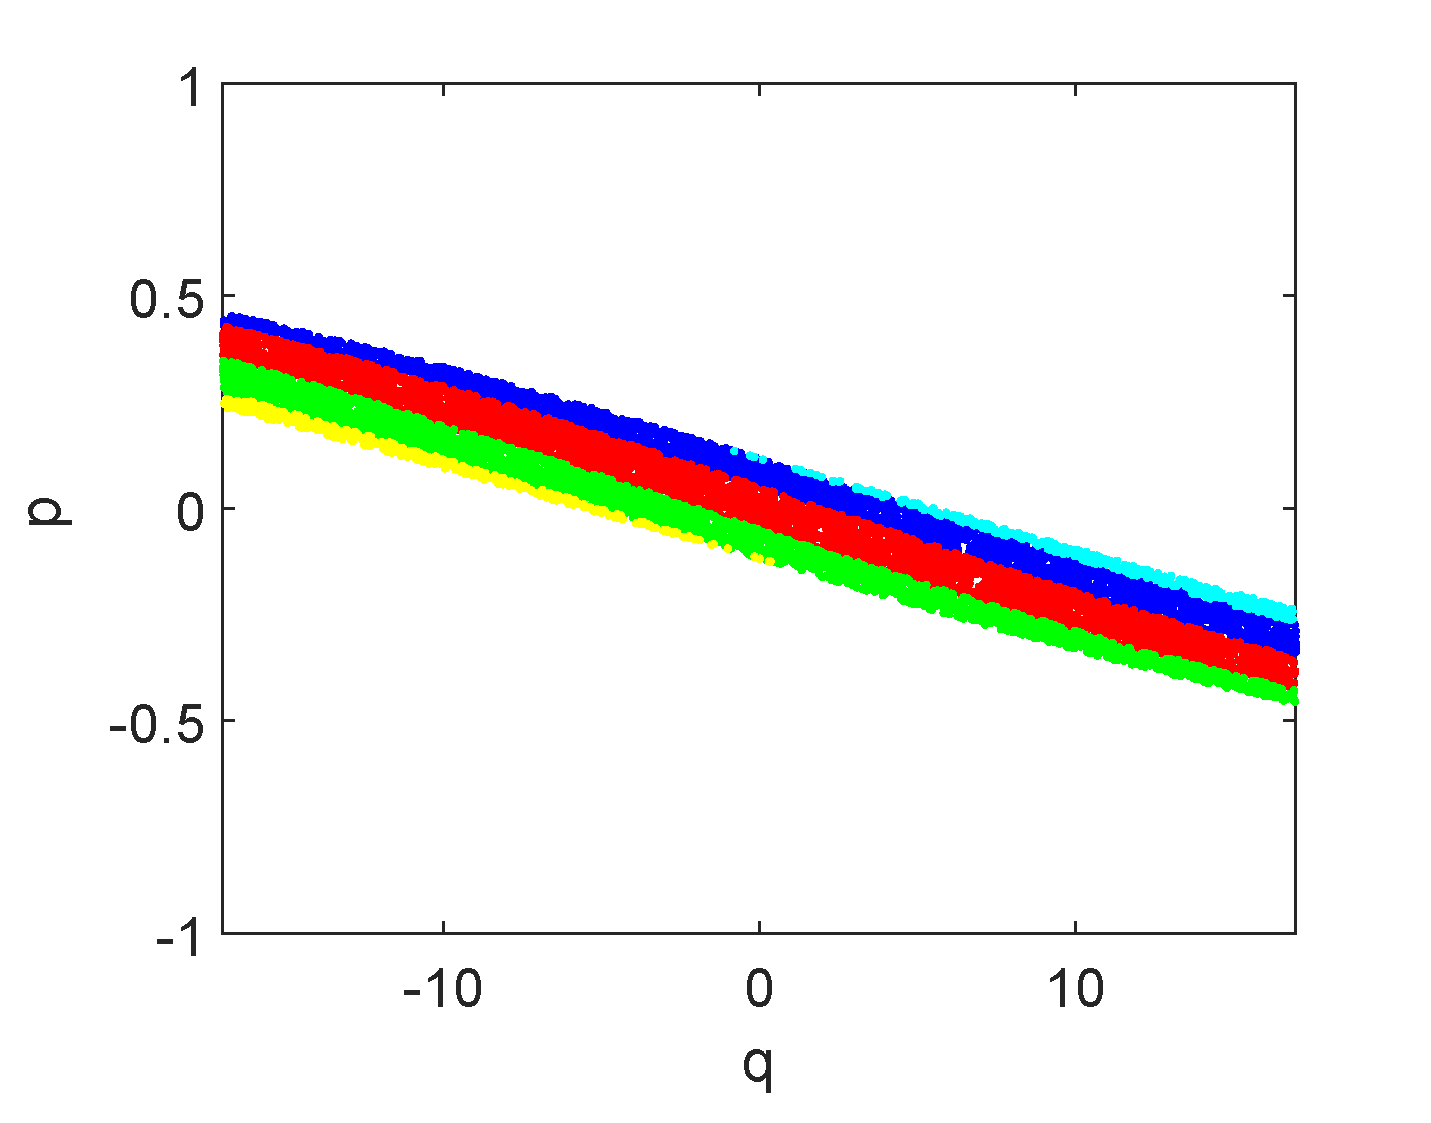
\includegraphics[width=\textwidth]{target_PS_cup.pdf}
  \caption{\textbf{Ray at the target PS of the system.}}
\label{fig:PS_intro}
 \end{minipage}
\end{figure}
PS ray tracing takes into account the \textit{path} followed by every ray, that is, the sequence of the optical components encountered by every ray traced.
Considering for every ray traced its corresponding path, we observe that the PS of the source and the target are partitioned into regions, each of them is formed by the rays that follow the same path. 
While the source PS is compleatly covered by the rays, the target PS can have some empty  The boundaries of the regions in target PS give important information about the output photometric variables because there the target luminance has a jump discontinuity from zero to a positive value. 
%LED light sources are close to Lambertian, i.e., they emit equal luminance in every direction \cite{taylor2000illumination}. For systems with a Lambertian source the boundaries of these regions give \textit{all} the information needed for computing the luminance and the intensity and, as a consequence, it is not required to trace rays that will be located in the interior of these regions.
%In the general case of a non-Lambertian source, a sample of rays inside 
The positive luminance regions should be considered over all the possible directions to provide the profile of the output luminance. 
Numerical integration gives the target intensity profile. Detecting the boundaries of the positive luminance regions, the computation of the photometric variables can be quickly computed without the need for tracing millions of rays which is instead necessary for conventional procedures such as MC and QMC ray tracing. We focus on two different procedures: phase space ray tracing and backward ray mapping in phase space.

\textit{Phase space ray tracing} is a forward method that employs the source and the target PS representation of the optical system. The key idea is to construct a nonuniform triangulation in PS such that more triangles are defined close to the discontinuity of the luminance. For the sake of simplicity, we construct the triangulation in source PS. The coordinates of the vertices of each triangle correspond to the coordinates of the rays traced that will be located close to the discontinuities of the luminance. In order to compute the target photometric variables, the boundaries of the positive luminance regions need to be calculated. 
%Assuming a Lambertian source, these boundaries give \textit{all} the information needed for the luminance and the intensity calculation. 
Therefore, we provide two different approaches to obtain an approximation of the boundaries at the source PS.

The first technique is based on $\alpha$-shapes. 
Given a triangulation in source PS (usually the Delanauy triangulation \cite{marsden2003texts}), the parameter $\alpha$ is used to decide which triangles have to be considered for the boundaries computation and which have to be removed. In general it is not easy to establish the value of parameter $\alpha$ that gives the desired boundary computation \cite{teichmann1998surface}. We develop a procedure based on \'{e}tendue conservation \cite{filosa2015new}. 

The second technique for the boundaries computation exploits the triangulation refinement explained above. The approximation of the boundaries in source PS is obtained by connecting the vertices on one side of the boundary between two regions, corresponding to rays that follow different paths.
%The $\alpha$-shapes method considers a triangulation (usually the Delanauy triangulation \cite{marsden2003texts}) of the set of points obtained from the triangulation refinement of the source PS. Then, the parameter $\alpha$ is used to decide which triangles have to be considered for the boundaries computation and which have to be removed. For every triangle the radius of its circumcircle is considered. If it is greater than $\alpha$, then the triangle is eliminated from the triangulation. Connecting the edges of the remaining triangles belonging to only one triangle, the $\alpha$-shape of the points cloud is found. In general it is not easy to establish the value of parameter $\alpha$ that gives the desired boundary computation \cite{teichmann1998surface}. We develop a procedure based on \'{e}tendue conservation \cite{filosa2015new}. \\ \indent The second technique for the boundaries computation exploits the triangulation refinement explained above. The approximation of the boundaries in source PS is obtained by connecting the vertices on one side of the boundary between two regions, corresponding to rays that follow different paths. The finer the triangulation, the more accurate the boundaries are. 
Etendue conservation is used to provide a stopping criterion for the triangulation refinement \cite{filosa2016ray, filosa2017phase}.  

Once the boundaries are calculated at the source PS, also the boundaries at the target are obtained (edge-ray principle, \cite{Ries:2}). Assuming a Lambertian source, the output intensity is calculated by only considering the rays located on these boundaries. 

Numerical results are provided using both $\alpha$-shapes and the triangulation refinement for several optical systems.
To validate the method, the intensities found are compared to both MC and QMC simulations. The results demonstrate that using PS ray tracing allows tracing far less rays than MC ray tracing to obtain an accurate approximation of the intensity profile. However, when using $\alpha$-shapes, the number of rays traced depends on the complexity of the design of the optical system. On the other hand, computing the boundaries employing the triangulation refinement, a speed of convergence proportional to the inverse of the number of rays traced is obtained for all the systems considered versus a speed of convergence proportional to the inverse of the square root of the number of rays traced obtained using MC ray tracing. Numerical simulations show that PS ray tracing based on the triangulation refinement gives speed advantages also comparable with QMC ray tracing when applied to some optical systems, while it is slower than QMC for some other systems.
PS ray tracing is therefore further improved by introducing the backward ray mapping method based on a ray mapping reconstruction in PS. 

\textit{Backward ray mapping in phase space} is first developed for systems formed by straight line segments. In this case the phase spaces of \textit{all} the lines that constitutes the system are considered. We assume that the optical lines are designed such that they can both receive and emit light while the source can only emit light and the target only receive it. Both source and target PS of each line are computed and only one PS is implemented for the source and the target. Concatenating all the phase spaces with two different maps, we are able to construct an inverse map from the target to the source. This explains the name \textit{concatenated backward ray mapping} for this method. Numerical results show that only the rays on the target PS that are located \textit{exactly} at the boundaries of the positive luminance regions are traced inside the system. The output intensity is computed integrating the luminance at the target PS. A comparison between concatenated backward ray mapping and QMC ray tracing demonstrates that our method computes the \textit{exact} intensity, reducing significantly the computational time. 

In order to extend the method to system formed also by curved line we use a different approach which employs the PS representation of the target of the optical system. Applying a bisection method combined with backward ray tracing we are able to construct the inverse map from the target to the source \textit{directly}. This allows tracing only the rays at the boundaries of the positive luminance regions \cite{filosa2017inverse}. From these rays the output intensity is calculated. We show in simulations that \textit{direct backward ray mapping} is more accurate and faster than QMC ray tracing.

Finally direct backward ray mapping is extended to systems with Fresnel reflections. In this case every ray incident on a Fresnel lens is split into a reflected and a refracted ray, each of them carry a fraction of the energy of the incident ray. This leads to a multitude of possible paths. 
%Direct backward ray mapping is applied considering every possible path separately. Given a path the rays located on the boundary of the corresponding region in target PS are traced from the target to the source. 
Numerical simulations show that direct backward ray mapping is able to detect \textit{all} the possible paths and to determine the boundaries of \textit{all} the positive luminance regions in target PS. Since, for Fresnel systems, the luminance is not constant at the target, a sample of rays inside those regions needs to be considered for calculating the luminance and the intensity profile.
\section{Outline of this thesis}
This work is organized in the following way.

In Chapter \ref{chap:Illumination optics} an overview of the physics of illumination optics is provided. After a short introduction of radiometric variables, the photometric counterparts are defined. The reflection and refraction laws are described and total internal reflection is discussed. A description of Fresnel reflection is included. In this chapter we follow the literature reported in \cite{hecht1998hecht, feynman2011feynman, feynman1964feynman}.

Chapter \ref{chap:raytracing} includes a discussion on classical ray tracing. First, we introduce the general case of MC and QMC methods which are very often used in numerical integration for approximating the integral of a given function. A mathematical formulation of both methods is given. Second MC and QMC ray tracing are discussed. They are based on a combination of MC and QMC procedures with ray tracing methods. We explain how to calculate the target intensity using these techniques, numerical results for a simple system show the convergence of the approximated intensities to the exact intensity by increasing the number of rays traced.

Chapter \ref{chap:PS} introduces the PS concept for two-dimensional optical systems. We show that the PS provides a complete description of optical systems. We explain how to construct the triangulation refinement on which PS ray tracing is based. The PS representation of the source and the target of a simple system (the two-faceted cup) shows that the phase spaces are divided into several regions formed by rays that follow the same path when they propagates through the system. Two techniques for calculating the boundaries of these regions are provided next. 
 
A method based on $\alpha$-shapes is presented in Chapter \ref{chap:boundaries_alpha}. A technique based on \'{e}tendue conservation is developed and numerical results for two different total internal reflection (TIR)-collimators are provided. For these systems also the target intensity in PS is calculated and it is compared with MC ray tracing. The chapter concludes with a discussion of the results obtained.

A different approach for the boundaries calculation which employs a triangulation refinement in source PS is provided in Chapter \ref{chap:triangulation}. The method is applied to three different systems: the two-faceted cup, a TIR-collimator and a parabolic reflector, numerical results are compared with both MC and QMC ray tracing.

Next, a second method based on ray mapping reconstruction from the target to the source is developed. Chapter \ref{chap:raymapping1} includes the description of concatenated backward ray mapping for systems formed by straight and reflective line segments. The target intensity is computed for two different optical systems: the two-faceted cup and a multifaceted cup. Numerical results are compared to QMC ray tracing. 

In Chapter \ref{chap:raymapping2} we present the direct backward ray mapping method which is an extension to systems formed by curved and refractive lines. A detailed explanation of the idea and the algorithm used are given. The results for the TIR-collimator and the parabolic reflector validate the method showing that it calculates the intensity correctly compared to QMC ray tracing. 

The research concludes with Chapter \ref{chap:fresnel} which discusses direct backward ray mapping applied to systems with Fresnel reflection. The theoretical explanation of the method is followed by numerical results applied to a system formed by the source, the target and a simple convex lens. We show in simulations that the boundaries of the positive luminance regions are calculated correctly. Finally, the profile of the luminance is obtained considering a sample of rays inside these regions and the intensity is given by integrating the luminance over all the possible positions. 

Chapter \ref{chap:conclusions} summaries the finding and presents discussions and insights for future prospective.
\clearpage{\pagestyle{empty}\cleardoublepage}
 